\documentclass[10pt,twocolumn,letterpaper]{article}

\usepackage{cvpr}
\usepackage{times}
\usepackage{epsfig}
\usepackage{graphicx}
\usepackage{amsmath}
\usepackage{amssymb}
\usepackage{subfigure}
\usepackage{epstopdf}
\usepackage{multirow}

% Include other packages here, before hyperref.

% If you comment hyperref and then uncomment it, you should delete
% egpaper.aux before re-running latex.  (Or just hit 'q' on the first latex
% run, let it finish, and you should be clear).
\usepackage[breaklinks=true,bookmarks=false]{hyperref}

\cvprfinalcopy % *** Uncomment this line for the final submission

\def\cvprPaperID{****} % *** Enter the CVPR Paper ID here
\def\httilde{\mbox{\tt\raisebox{-.5ex}{\symbol{126}}}}

% Pages are numbered in submission mode, and unnumbered in camera-ready
%\ifcvprfinal\pagestyle{empty}\fi
\setcounter{page}{4321}
\begin{document}

%%%%%%%%% TITLE
\title{CMPE 264 - Project Assignment 1}

\author{Yanan Xie\\
{\tt\small yaxie@ucsc.edu}
% For a paper whose authors are all at the same institution,
% omit the following lines up until the closing ``}''.
% Additional authors and addresses can be added with ``\and'',
% just like the second author.
% To save space, use either the email address or home page, not both
\and
Ziqiang Wang\\
{\tt\small secondauthor@i2.org}
}

\maketitle
%\thispagestyle{empty}

%%%%%%%%% ABSTRACT

%%%%%%%%% BODY TEXT
\section{Camera radiometric calibration}

In this section, we describe how we take pictures and estimate the relationship between B and T.

%-------------------------------------------------------------------------
\subsection{Taking pictures}

In order to simulate a surface with uniform radiance, we put a scratch paper on the table. Then, we took 9 pictures with a Canon 5D Mark II(DSLR) and a 40mm lens. A tripod was utilized to stabilize the camera. ISO was set to 100. F-number of the lens was set to 4. The exposure times of those 9 pictures are $1/25s$, $1/30s$, $1/40s$, $1/50s$, $1/60s$, $1/80s$, $1/100s$, $1/125s$, and $1/160s$ respectively. Pictures are all JPEG format. Figure \ref{fig:samplepicture} shows a picture taken with $T = 1/30s$ as an example. \\

Sample area was chosen to be the center of the picture with a size $100\times 100$. As shown in figure \ref{fig:sampler}, \ref{fig:sampleg} and \ref{fig:sampleb}, the sampled areas are not saturated in any channels. And the strips confirmed that the pictures were taken very stably.

\begin{figure}[bhp]
\includegraphics[width=\columnwidth]{images/_MG_6277}
\caption{T = 1/30s}

\label{fig:samplepicture}
\end{figure}


\begin{figure}[t]
\centering
\subfigure[$T=1/160s$]{
\includegraphics[width=.3\columnwidth]{images/samples/0_2}
}
\subfigure[$T=1/125s$]{
\includegraphics[width=.3\columnwidth]{images/samples/1_2}
}
\subfigure[$T=1/100s$]{
\includegraphics[width=.3\columnwidth]{images/samples/2_2}
}
\subfigure[$T=1/80s$]{
\includegraphics[width=.3\columnwidth]{images/samples/3_2}
}
\subfigure[$T=1/60s$]{
\includegraphics[width=.3\columnwidth]{images/samples/4_2}
}
\subfigure[$T=1/50s$]{
\includegraphics[width=.3\columnwidth]{images/samples/5_2}
}
\subfigure[$T=1/40s$]{
\includegraphics[width=.3\columnwidth]{images/samples/6_2}
}
\subfigure[$T=1/30s$]{
\includegraphics[width=.3\columnwidth]{images/samples/7_2}
}
\subfigure[$T=1/25s$]{
\includegraphics[width=.3\columnwidth]{images/samples/8_2}
}

\caption{Sample areas of Channel R}
\label{fig:sampler}
\end{figure}

\begin{figure}[t]
\centering
\subfigure[$T=1/160s$]{
\includegraphics[width=.3\columnwidth]{images/samples/0_1}
}
\subfigure[$T=1/125s$]{
\includegraphics[width=.3\columnwidth]{images/samples/1_1}
}
\subfigure[$T=1/100s$]{
\includegraphics[width=.3\columnwidth]{images/samples/2_1}
}
\subfigure[$T=1/80s$]{
\includegraphics[width=.3\columnwidth]{images/samples/3_1}
}
\subfigure[$T=1/60s$]{
\includegraphics[width=.3\columnwidth]{images/samples/4_1}
}
\subfigure[$T=1/50s$]{
\includegraphics[width=.3\columnwidth]{images/samples/5_1}
}
\subfigure[$T=1/40s$]{
\includegraphics[width=.3\columnwidth]{images/samples/6_1}
}
\subfigure[$T=1/30s$]{
\includegraphics[width=.3\columnwidth]{images/samples/7_1}
}
\subfigure[$T=1/25s$]{
\includegraphics[width=.3\columnwidth]{images/samples/8_1}
}

\caption{Sample areas of Channel G}
\label{fig:sampleg}
\end{figure}

\begin{figure}[t]
\centering
\subfigure[$T=1/160s$]{
\includegraphics[width=.3\columnwidth]{images/samples/0_0}
}
\subfigure[$T=1/125s$]{
\includegraphics[width=.3\columnwidth]{images/samples/1_0}
}
\subfigure[$T=1/100s$]{
\includegraphics[width=.3\columnwidth]{images/samples/2_0}
}
\subfigure[$T=1/80s$]{
\includegraphics[width=.3\columnwidth]{images/samples/3_0}
}
\subfigure[$T=1/60s$]{
\includegraphics[width=.3\columnwidth]{images/samples/4_0}
}
\subfigure[$T=1/50s$]{
\includegraphics[width=.3\columnwidth]{images/samples/5_0}
}
\subfigure[$T=1/40s$]{
\includegraphics[width=.3\columnwidth]{images/samples/6_0}
}
\subfigure[$T=1/30s$]{
\includegraphics[width=.3\columnwidth]{images/samples/7_0}
}
\subfigure[$T=1/25s$]{
\includegraphics[width=.3\columnwidth]{images/samples/8_0}
}

\caption{Sample areas of Channel B}
\label{fig:sampleb}
\end{figure}

\subsection{Discovering the relation between $B$ and $T$}

$B$ is estimated by the average value of the sampled area $B'$. We calculate $B'$ in RGB channels independently in order to solve the non-linear function between $B'$ and $B$. \\

We assume $B = k\frac{B'}{255}^gT$ following the assumption given by the instruction. However, we did add a divider under $B'$ to normalize $B$ , so that we can compare MSEs(mean squared error) among different values of $g$.



\begin{figure}[t]
\centering
\subfigure[$g=1.0$]{
\includegraphics[width=.47\columnwidth]{images/rchannel10}
}
\subfigure[$g=3.5$]{
\includegraphics[width=.47\columnwidth]{images/rchannel35}
}
\subfigure[$g=6.0$]{
\includegraphics[width=.47\columnwidth]{images/rchannel60}
}
\subfigure[$g=8.5$]{
\includegraphics[width=.47\columnwidth]{images/rchannel85}
}

\caption{$\frac{B'}{255}^g$ and $T$ in Channel R}
\label{fig:sampleb}
\end{figure}

\begin{figure}[t]
\centering
\subfigure[$g=1.0$]{
\includegraphics[width=.47\columnwidth]{images/gchannel10}
}
\subfigure[$g=1.5$]{
\includegraphics[width=.47\columnwidth]{images/gchannel25}
}
\subfigure[$g=2.0$]{
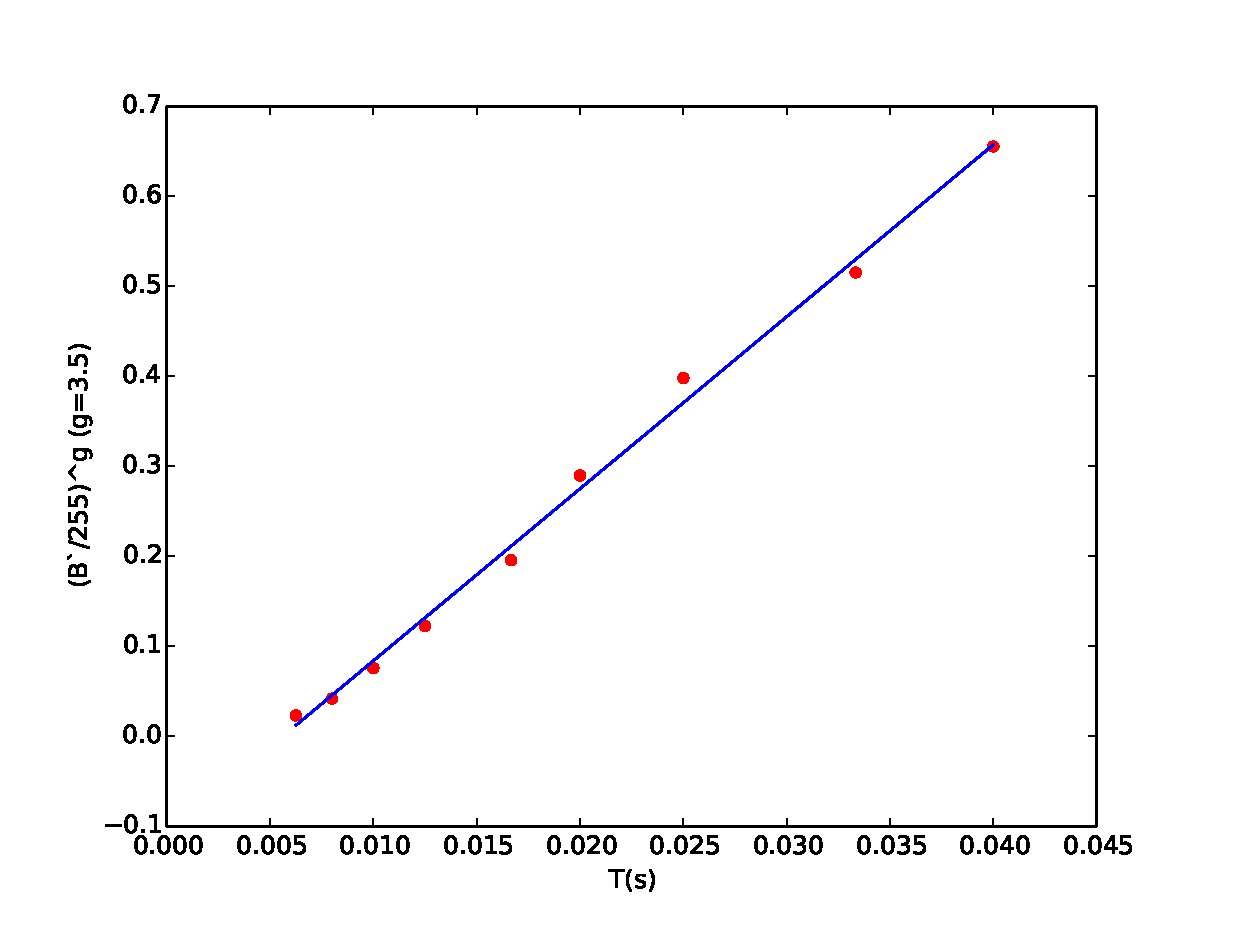
\includegraphics[width=.47\columnwidth]{images/gchannel35}
}
\subfigure[$g=2.5$]{
\includegraphics[width=.47\columnwidth]{images/gchannel45}
}

\caption{$\frac{B'}{255}^g$ and $T$ in Channel G}
\label{fig:sampleb}
\end{figure}
\begin{figure}[t]
\centering
\subfigure[$g=1.0$]{
\includegraphics[width=.47\columnwidth]{images/bchannel10}
}
\subfigure[$g=1.5$]{
\includegraphics[width=.47\columnwidth]{images/bchannel15}
}
\subfigure[$g=2.0$]{
\includegraphics[width=.47\columnwidth]{images/bchannel20}
}
\subfigure[$g=2.5$]{
\includegraphics[width=.47\columnwidth]{images/bchannel25}
}

\caption{$\frac{B'}{255}^g$ and $T$ in Channel B}
\label{fig:sampleb}
\end{figure}

\begin{table}[]
\caption{Linear regression results}
\centering
\begin{tabular}{|c|c|c|c|}
\hline
\hline
Channel &  g  &  coefficient & mean squared error  \\
\hline
 \multirow{4}{*}{R} &  1.0  & 15.507411  &  0.005077  \\
 \cline{2-4}
&3.5&27.524782&0.003586\\
 \cline{2-4}
&6.0&28.342635&\textbf{0.001135}\\
 \cline{2-4}
&8.5&26.893380&0.002171\\
 \hline
 \multirow{4}{*}{G} &  1.0 &15.688164&0.002517\\
 \cline{2-4}
&2.5&20.172157&0.000763\\
 \cline{2-4}
&3.5&19.114863&\textbf{0.000191}\\
 \cline{2-4}
&4.5&17.217906&0.000381\\
 \hline
 \multirow{4}{*}{B} &1.0&13.43860314&0.000583\\
 \cline{2-4}
&1.5&12.83838657&0.000202\\
 \cline{2-4}
&2.0&11.11682836&\textbf{0.000067}\\
 \cline{2-4}
&2.5&9.18619509&0.000077\\
 \hline

\end{tabular}
\label{tab:linear}
\end{table}




\end{document}
